\chapter{Introduzione}
\label{Introduzione}
%
\section{Obiettivi}
La motivazione di questa tesi sta nella trovata collaborazione tra il Dipartimento di Ingegneria Industriale dell'Università di Trento e AnteMotion S.r.l., azienda specializzata in realtà virtuale e simulazione \textit{multibody} per il campo \textit{automotive}. In particolare il modello di veicolo e pneumatico precedentemente studiati da \citeauthor{Larcher} in \cite{Larcher} saranno integrati nel simulatore di guida in tempo reale di AnteMotion. Pertanto, lo sviluppo dei modelli è stato finalizzato a minimizzare i tempi di compilazione massimizzando invece l'accuratezza. La necessità di sviluppare un algoritmo che calcoli i parametri dell'interazione tra terreno, rappresentato con una \textit{mesh} triangolare, e pneumatico, rappresentato come un disco indeformabile, getta le basi per il lavoro svolto.
%
\section{Il problema}
La simulazione risolve alcuni dei problemi relativi al mondo della progettazione in modo sicuro ed efficiente, senza la necessità di costruire un prototipo dell'oggetto fisico. A differenza della modellazione fisica, che può coinvolgere il sistema reale o una copia in scala di esso, la simulazione è basata sulla tecnologia digitale e utilizza algoritmi ed equazioni per rappresentare il mondo reale al fine di imitare l'esperimento reale. Ciò comporta diversi vantaggi in termini di tempo, costi e sicurezza. Infatti, il modello digitale può essere facilmente riconfigurato e analizzato, mentre questo è solitamente impossibile o troppo oneroso del punto di vista di tempi e/o costi da fare con il sistema reale \cite{Anu}.

Al giorno d'oggi esistono numerosi modelli di veicolo e pneumatico. Certamente, più semplice è il modello più veloce è la risoluzione delle equazioni costituenti quindi, a seconda delle applicazioni, dev'essere scelto il modello con la giusta complessità. Per la maggior parte delle applicazioni di guida autonoma, un modello semplice è sufficiente per caratterizzare con un livello di dettaglio sufficiente il comportamento del veicolo, e poiché queste analisi sono molto spesso fatte con l'ausilio di \ac{HIL}, il modello dinamico del veicolo dev'essere risolto in tempo reale con tipico passo di tempo di un millisecondo. Il vincolo di esecuzione in tempo reale implica la scelta un modello di veicolo che sia velocemente risolvibile, ciò significa che i modelli semplici con pochi parametri, di solito modelli lineari a due ruote, sono particolarmente adatti per questo tipo di applicazioni. Tuttavia, ci sono alcune situazioni che richiedono modelli più dettagliati, come ad esempio l'azione prodotta da un \ac{ADAS}, ovvero una manovra di sicurezza come l'elusione degli ostacoli o una frenata di emergenza, poiché il veicolo è spinto nella maggior parte dei casi al limite delle sue prestazioni \cite{impacts}. In queste condizioni di guida si devono tenere conto di molti fattori come ad esempio il comportamento degli pneumatici, che si sposta nella regione non lineare e i fenomeni transitori non sono più trascurabili. Questo implica la necessità di utilizzare un modello più dettagliato di quello utilizzato per la guida in condizioni \textit{standard}.

L'accuratezza dinamica del modello è di grande rilevanza per ricavare previsioni realistiche delle prestazioni del veicolo e del sistema di controllo. È importante notare che modellare in modo esaustivo tutti i sistemi di un'auto sarebbe un compito estremamente arduo e a volte anche impossibile. Esistono quindi modelli empirici come il modello della \textit{Magic Formula} di Hans Pacejka, che cerca di imitare il reale comportamento del sistema. Il calcolo dei parametri di questo tipo di modelli richiede l'interpolazione di un insieme di dati di grandi dimensioni, e può quindi essere numericamente inefficiente o comunque troppo oneroso in termini di tempo.
Lo scopo di questo lavoro si collega a quello già svolto da \citeauthor{Larcher} in \cite{Larcher}, dove grazie a un modello di veicolo completo con 14 gradi di libertà ha fornito un modello in grado di catturare con un livello di dettaglio appropriato il comportamento del veicolo quando viene spinto alle massime prestazioni. La necessità di calcolare in tempo reale i parametri di input per il modello di ruota scelto da \cite{Larcher} definisce l'obiettivo di questo lavoro. Ovvero di avere una libreria scritta in \texttt{C++}, che con alcuni semplici parametri in input come la denominazione \ac{ETRTO} dello pneumatico e la posizione nello spazio, calcola i dati relativi all'interazione pneumatico strada quali il punto di contatto virtuale e l'inclinazione locale del piano strada. Il tutto cercando di minimizzare i tempi di compilazione.
%
\section{Convenzioni e Notazioni}
\label{Notazioni}
%
\subsection{Sistemi di Riferimento}
La convenzione utilizzata per definire gli assi del sistema di riferimento della vettura è la \ac{ISO} 8855.

\begin{figure}[h!]
	\centering
	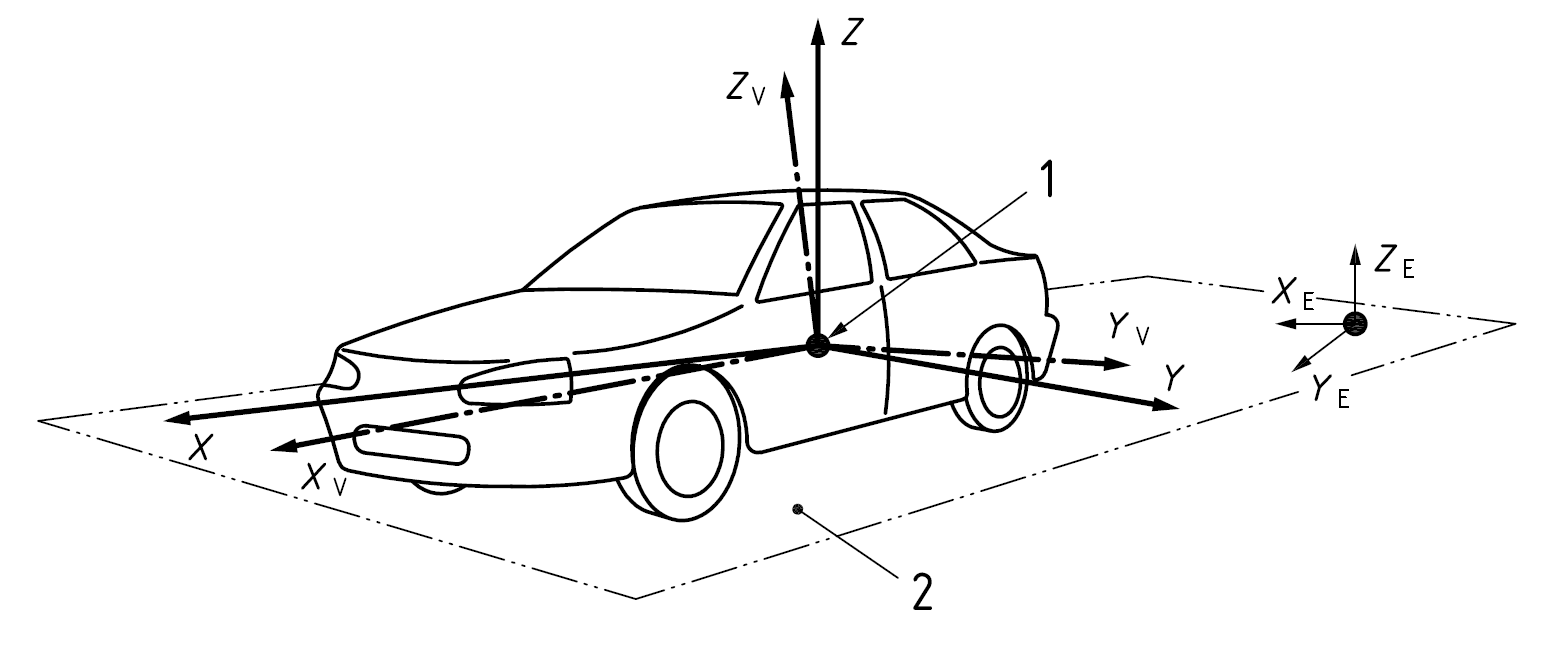
\includegraphics[width=0.8\linewidth]{Figures/iso_convention}
	\caption{Rappresentazione degli assi del sistema di riferimento della vettura secondo la convenzione ISO-V.}
	\label{isoconventionv}
\end{figure}

\noindent
Il sistema di riferimento della ruota è conforme alla convenzione \ac{ISO}-V, la cui disposizione degli assi è illustrata nella \figurename{ \ref{isoconventionc}}. L'origine del sistema di riferimento del vettore ruota è posta in corrispondenza del centro della ruota mentre posizione e orientamento relativi rispetto al sistema di riferimento del telaio sono definiti attraverso il modello della sospensione descritto in \cite{Larcher}.

\begin{figure}[h!]
	\centering
	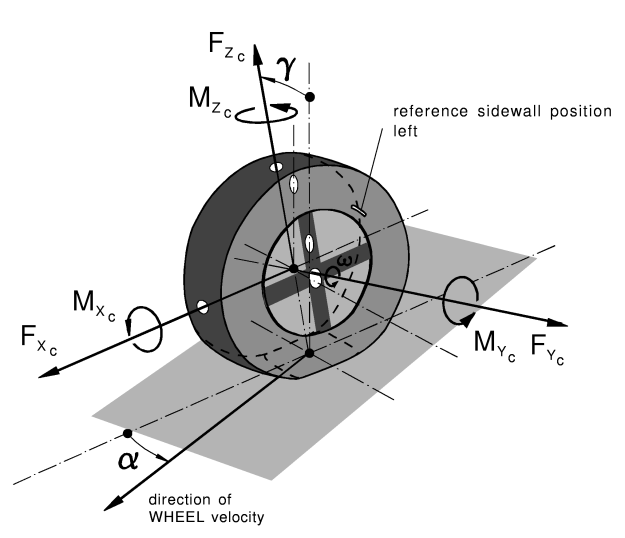
\includegraphics[width=0.7\linewidth]{Figures/iso_convention_wheel}
	\caption{Rappresentazione degli assi  del sistema di riferimento dello pneumatico secondo la convenzione ISO-C.}
	\label{isoconventionc}
\end{figure}
%
\subsection{Matrice di Trasformazione}
Per descrivere sia l'orientamento che la posizione di un sistema di assi nello spazio, viene introdotta la matrice roto-traslazione, chiamata anche matrice di trasformazione. Questa notazione permette di impiegare le operazioni matrice-vettore per l'analisi di posizione, velocità e accelerazione. La forma generale di una matrice di trasformazione è del tipo:
%
\begin{equation}
T_m = \left[
\begin{array}{ccc|c}
& & & O_{mx}\\
\multicolumn{3}{c|}{\multirow{3}{*}{\raisebox{20mm}{\scalebox{1.5}{$[R_m]$}}}} & O_{my}\\
& & & O_{mz}\\ \hline
0 & 0 & 0 & 1
\end{array}\right]
\end{equation}\\
%
dove $R_m$ è la matrice di rotazione $3 \times 3$ del sistema di riferimento in movimento e $O_{mx}$, $O_{my}$ e $O_{mz}$ sono le coordinate della sua origine nel sistema di riferimento assoluto o nativo.

L'introduzione dell'elemento fittizio 1 nel vettore della posizione di origine e la successiva spaziatura interna zero della matrice rende possibili le moltiplicazioni matrice-vettore, rendendo la matrice di trasformazione una notazione compatta e conveniente per la descrizione dei sistemi di riferimento. Si noti che per i vettori, le informazioni traslazionali vengono trascurate imponendo l'elemento fittizio pari a 0.